%% Course preprint in IJCAI style.
%% Not submitted to or accepted by IJCAI.
%%
%% To build with the OFFICIAL style: download the IJCAI-ECAI 2026 author kit
%% (https://www.ijcai.org/authors_kit) and copy ijcai26.sty and named.bst into this
%% folder. Without them, this file falls back to a plain two-column layout so it
%% still compiles.
\documentclass{article}
\pdfpagewidth=8.5in
\pdfpageheight=11in

\IfFileExists{ijcai26.sty}{\usepackage{ijcai26}}{%
  \usepackage[letterpaper,margin=0.75in,columnsep=0.25in]{geometry}%
  \AtBeginDocument{\twocolumn}}

\usepackage{times}
\IfFileExists{soul.sty}{\usepackage{soul}}{}
\usepackage{url}
\usepackage[hidelinks]{hyperref}
\usepackage[utf8]{inputenc}
\usepackage[small]{caption}
\usepackage{graphicx}
\usepackage{amsmath}
\usepackage{amssymb}
\usepackage{booktabs}
\usepackage{xcolor}
\urlstyle{same}

\providecommand{\affiliations}{\\}
\newcommand{\todo}[1]{\textcolor{red}{\textbf{[TODO: #1]}}}
\newcommand{\Pc}{P(\mathrm{C})}

\title{Cloud Cost Agent:\\Ignore, Investigate, Limit, or Report? A Cost-Aware Bayesian Agent for Unexplained Cloud Cost Spikes}

\author{
Vaishnavi
\affiliations
Independent DevOps Engineer, Karnataka, India
% \emails
% your-email@example.com
}

\begin{document}

\maketitle
\renewcommand{\thefootnote}{}\footnotetext{Course preprint (Week 1 AI-Native project). Not submitted to or accepted by IJCAI; the IJCAI format is used for style only.}\renewcommand{\thefootnote}{\arabic{footnote}}

\begin{abstract}
When a cloud bill jumps, an engineer must act before knowing the cause: normal variation, a planned job, wasted resources, or a security compromise. We present a small agent that observes one daily AWS cost line item and its 7-day history, keeps a probability over these four hidden causes, and chooses to ignore, report, or limit the cost, optionally paying for an investigation first. Actions are chosen by minimum expected dollar cost, and investigation is chosen by its value of information. We test the agent on 40-case sets built by injecting labeled anomalies into mock AWS billing data, and repeat the test on 30 random case sets. Compared with a threshold alert, the cost-aware agent (v2) lowers mean decision cost from \$17{,}781 to \$4{,}038 per 40 cases and missed compromises from 2.47 to 0.10, but it raises more false alarms (14.2 vs.\ 5.8). Choosing the most likely cause performs worst of all policies. An ablation shows that a free owner-tag check gives the largest gain and also causes a new failure: untagged planned jobs are limited as if they were attacks. All results are from simulation, and the cases were generated with assumptions similar to the agent's own, so they are optimistic.
\end{abstract}

%% ---------------------------------------------------------------
\section{Introduction}

Unexpected cloud spend is a common operational problem. Practitioners describe it as \emph{anomaly management}~\cite{finops2026framework}, and cloud providers offer anomaly alerts~\cite{aws2026anomaly}. An alert, however, only says that a cost is unusual. It does not say \emph{why}, and the right response depends on the cause. Ignoring a compromise (for example, leaked keys running crypto-mining instances) lets the bill grow every hour. Shutting down a planned production job causes a self-inflicted outage. Sending every alert to a human creates alert fatigue.

We study this as a decision problem under incomplete information:

\begin{quote}
\emph{The agent observes a daily AWS cost line item (service, region, usage, cost) and that service's recent history. It must choose to ignore, investigate, limit, or report the cost because the cause of the cost change is not known.}
\end{quote}

Our contributions are small and specific:
(1)~a four-state Bayesian agent with an explicit dollar cost table and a value-of-information rule for investigating;
(2)~a test on simulated cases with a threshold baseline, two policy versions, a holdout set, 30 random case sets, an ablation, a sensitivity analysis, and a calibration check;
(3)~a named failure analysis, including one failure that our own design change introduced.
Code and data:\\ \url{https://github.com/Vaishnavi1607678/Cloud-Cost-Agent}.

%% ---------------------------------------------------------------
\section{Related Work and User Discussions}

\paragraph{Anomaly detection.} Classical methods flag points that differ from an expected pattern~\cite{chandola2009anomaly}. Streaming methods such as Robust Random Cut Forest~\cite{guha2016rrcf} and seasonal statistical tests for cloud metrics~\cite{hochenbaum2017automatic} detect \emph{that} something is unusual. AWS Cost Anomaly Detection~\cite{aws2026anomaly} applies this idea to billing. These methods answer ``is it unusual?'' but not ``what should we do?''. We could not run AWS Cost Anomaly Detection on our mock data, so we use a z-score threshold as a stand-in baseline.

\paragraph{Cost-sensitive decisions.} When errors have different costs, the best decision minimizes expected cost rather than error rate~\cite{elkan2001foundations}. Deciding whether to collect more evidence before acting is the value-of-information problem~\cite{howard1966information}. Our agent combines both ideas in a very small setting.

\paragraph{User discussions.} At the time of this draft, the public discussions on Reddit and X had not yet produced answers that changed the design. The questions being taken to practitioners come directly from the failure analysis: (a)~do stolen keys appear as a known user in CloudTrail (F3)? (b)~would practitioners allow an automatic stop of an untagged resource (F7)? (c)~how many cost alerts per week before a team ignores them (the cost of Report)? (d)~is \$5{,}000 a realistic cost for a missed compromise?

%% ---------------------------------------------------------------
\section{Agent Design}

\paragraph{Input.} One daily row (service, region, usage type, usage amount, cost) and the previous 7 days for the same service.

\paragraph{Hidden states.} $S \in \{\mathrm{N}, \mathrm{P}, \mathrm{W}, \mathrm{C}\}$: Normal variation, Planned spike, Waste or misconfiguration, Compromise.

\paragraph{Evidence.} Free evidence: the spike level (\emph{low} $<1.5\times$, \emph{med} $<3\times$, \emph{high} $\geq 3\times$ the 7-day median) and whether the region is new. In v2, the spike uses $\max$(cost ratio, usage ratio) and the resource owner tag is also free (a tags API call). Paid evidence (\emph{Investigate}, \$25 of engineer time): whether CloudTrail shows a known launcher, and whether a change ticket exists.

\paragraph{Actions.} \emph{Ignore}; \emph{Report} (send to a human); \emph{Limit} (budget action or scale-down); and \emph{Investigate}, which is followed by one of the other three. In this study, actions are \emph{selected and logged} but not executed against a real AWS account.

\paragraph{Cost.} Table~\ref{tab:cost} gives our estimated cost of each action under each state. These values are assumptions; Section~\ref{sec:results} tests how sensitive the results are to them.

\begin{table}[t]
\centering
\small
\begin{tabular}{lrrrr}
\toprule
Action & Normal & Planned & Waste & Compromise \\
\midrule
Ignore & 0 & 0 & 400 & \textbf{5{,}000} \\
Report & 50 & 50 & 40 & 600 \\
Limit & 300 & \textbf{1{,}500} & 60 & 100 \\
\bottomrule
\end{tabular}
\caption{Estimated decision cost (US\$). Investigate adds \$25.}
\label{tab:cost}
\end{table}

\paragraph{Human reasoning function.} The agent \emph{changes its belief after new evidence} using Bayes' rule, and it decides whether new evidence is worth paying for.

\paragraph{Stakeholders.} The FinOps or finance team owns the budget, the security team owns compromise response, and service owners pay the cost of a wrong Limit. On-call engineers pay the cost of every Report.

\paragraph{Feedback (v2).} After each decision the true state is revealed, and the agent updates its likelihood tables with pseudo-counts (Section~\ref{sec:prob}).

%% ---------------------------------------------------------------
\section{Probability Model and Decision Rule}
\label{sec:prob}

The belief starts from a prior $P(\mathrm{N}) = 0.80$, $P(\mathrm{P}) = P(\mathrm{W}) = 0.08$, $\Pc = 0.04$, and is updated for each piece of evidence $e$ under a naive-Bayes assumption:
\begin{equation}
P(s \mid e_{1:k}) = \frac{P(s)\prod_{i=1}^{k} P(e_i \mid s)}{\sum_{s'} P(s')\prod_{i=1}^{k} P(e_i \mid s')}.
\end{equation}
The likelihoods are our estimates (for example, $P(\text{high} \mid \mathrm{C}) = 0.75$, $P(\text{tag missing} \mid \mathrm{C}) = 0.80$, $P(\text{tag missing} \mid \mathrm{N}) = 0.10$). The action with the lowest expected cost is chosen:
\begin{equation}
a^{*} = \arg\min_{a \in \{\mathrm{Ignore},\mathrm{Report},\mathrm{Limit}\}} \sum_{s} P(s \mid e)\, c(a, s).
\end{equation}
The agent investigates when the expected cost after seeing the paid clues $o$ is lower than acting now:
\begin{equation}
\begin{split}
& c_{\mathrm{inv}} + \sum_{o} P(o \mid e)\, \min_{a} \sum_{s} P(s \mid e, o)\, c(a,s) \\
& \qquad < \min_{a} \sum_{s} P(s \mid e)\, c(a,s).
\end{split}
\end{equation}

\paragraph{Thresholds.} From Table~\ref{tab:cost}, Report is cheaper than Ignore whenever $360\,P(\mathrm{W}) + 4{,}400\,\Pc > 50\,[P(\mathrm{N}) + P(\mathrm{P})]$, so in practice the agent reports once $\Pc$ exceeds about 1\%. Limit beats Report only if $500\,\Pc > 250\,P(\mathrm{N}) + 1{,}450\,P(\mathrm{P}) + 20\,P(\mathrm{W})$. In v2, a guard also requires $\Pc \geq 0.5$ before an automatic Limit; otherwise the case is reported.

\paragraph{Learning (v2).} Each binary likelihood $P(e{=}1 \mid s)$ is stored as Beta pseudo-counts $(\alpha_s, \beta_s) = (10p, 10(1{-}p))$; after feedback with true state $s$, the observed outcome's count increases by one. The spike likelihoods use Dirichlet counts in the same way. The prior is not learned, because the test mix is not a real base rate.

\paragraph{Worked example.} For the most expensive real row in the data (Lambda, 2025-07-10, $6.5\times$ the median, known region, unlabeled), the belief is $(0.36, 0.33, 0.22, 0.10)$ and the agent reports (expected cost \$100.5). If the owner tag is missing, $\Pc$ rises to 0.33 and investigating becomes worthwhile; if CloudTrail then shows an unknown launcher and no ticket, $\Pc = 0.74$ and the agent limits. The full record is in the repository.

%% ---------------------------------------------------------------
\section{Test Method}

\paragraph{Data.} Mock AWS billing data: 150 daily rows, 5 services (EC2, S3, Lambda, RDS, CloudFront), July 2025. It has no labels, and its price per unit and region change randomly from day to day.

\paragraph{Cases.} Each case takes a real row as ``today'' and its 7 previous days as history. Normal cases are left unchanged. Planned, Waste, and Compromise cases multiply usage and cost by $2$--$5\times$, $1.5$--$3.5\times$, and $3$--$10\times$ respectively; 70\% of compromises move to an unused region. Clue values are drawn from per-state rates. Each set has 40 cases: 14 Normal, 10 Planned, 9 Waste, 7 Compromise.

\paragraph{Protocol.} Labels are stored in a separate file and revealed only after each decision. We use a development set (seed 42) for v1 and its failure analysis, a \emph{holdout} set (seed 2026) created after v2 was designed, and 30 further random sets (seeds 1000--1029) for robustness, ablation, sensitivity, and calibration.

\paragraph{Policies.} \emph{Baseline}: Report if cost exceeds the 7-day mean by more than 2 standard deviations, else Ignore. \emph{Baseline+usage}: Report if the z-score of cost \emph{or} usage exceeds 2; it uses the same usage information as v2. \emph{A}: act on the most probable state. \emph{B}: minimum expected cost. \emph{v1 (C)}: B plus value-of-information investigation. \emph{v2}: C plus the usage ratio, a free owner tag, the Limit guard, and learning.

\paragraph{Metrics.} The correct action is Ignore for N and P, Report for W, and Limit for C. We report total decision cost, recall and false alarms for ``problem'' (W or C) vs.\ ``alert'' (Report or Limit), missed compromises, wrong Limits on N or P, human-review rate, the confusion matrix, Brier score, and calibration.

%% ---------------------------------------------------------------
\section{Results}
\label{sec:results}

\paragraph{Development set (v1).} The baseline cost \$19{,}860 and missed 3 of 7 compromises. Policy A was the \emph{worst} (\$31{,}800; 5 of 7 compromises missed): compromise is rare, so it is almost never the most probable state, even when it is the most expensive one to miss. Policy C cost \$8{,}605.

\paragraph{Holdout and robustness.} On the holdout set, total cost was \$21{,}090 (baseline), \$6{,}260 (v1), and \$4{,}080 (v2). Table~\ref{tab:main} and Figure~\ref{fig:box} show the 30-set results. v2 was cheaper than v1 in 25 of 30 sets (two-sided sign test, $p = 0.0003$). Giving the threshold baseline the same usage information lowers its cost to \$12{,}214, still about three times v2's.

\begin{table}[t]
\centering
\small
\setlength{\tabcolsep}{4pt}
\begin{tabular}{lrrrr}
\toprule
Mean per 40 cases & Base & Base+u & v1 (C) & v2 \\
\midrule
Total cost (\$) & 17{,}781 & 12{,}214 & 6{,}656 & \textbf{4{,}038} \\
Recall & 0.49 & 0.69 & 0.76 & \textbf{0.90} \\
Missed compromises & 2.47 & 1.33 & 0.57 & \textbf{0.10} \\
False alarms & \textbf{5.8} & 9.1 & 8.7 & 14.2 \\
Wrong Limits (N, P) & \textbf{0.00} & \textbf{0.00} & 0.03 & 0.20 \\
Human-review rate & \textbf{0.34} & 0.50 & 0.38 & 0.57 \\
Investigation rate & 0.00 & 0.00 & 0.50 & 0.19 \\
\bottomrule
\end{tabular}
\caption{Results over 30 random case sets (seeds 1000--1029).}
\label{tab:main}
\end{table}

\begin{figure}[t]
\centering
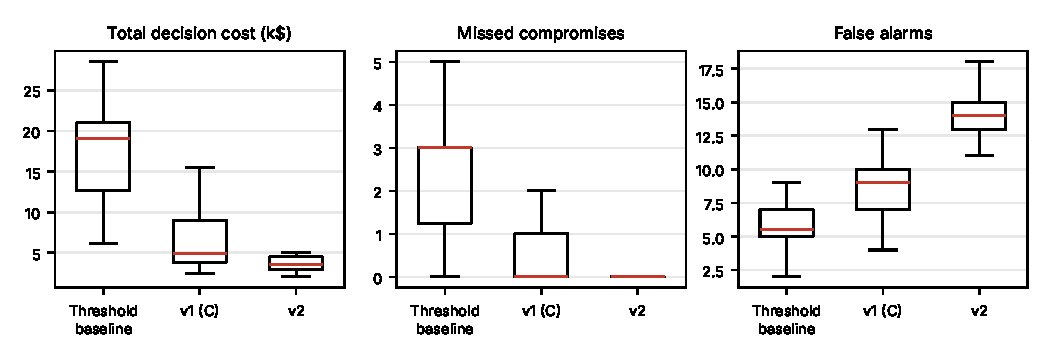
\includegraphics[width=\columnwidth]{figures/results_boxplot.pdf}
\caption{Distribution over 30 case sets of total decision cost, missed compromises, and false alarms.}
\label{fig:box}
\end{figure}

\paragraph{Ablation.} Table~\ref{tab:abl} adds one v2 change at a time (no learning). The free owner tag gives the largest reduction in missed compromises but raises wrong Limits from 0.03 to 0.20. The 50\% Limit guard alone did not prevent wrong Limits and increased cost. Learning reduced false alarms (15.7 to 14.2) but did not reduce cost (\$3{,}838 to \$4{,}038); 40 cases are too few to learn much.

\begin{table}[t]
\centering
\small
\begin{tabular}{lrrr}
\toprule
Variant & Cost (\$) & Missed C & Wrong Limit \\
\midrule
None (= v1 C) & 6{,}656 & 0.57 & 0.03 \\
+ usage ratio & 4{,}732 & 0.23 & 0.03 \\
+ free owner tag & 4{,}502 & 0.10 & 0.20 \\
+ Limit guard & 7{,}073 & 0.57 & 0.03 \\
All three & 3{,}838 & 0.03 & 0.23 \\
\bottomrule
\end{tabular}
\caption{Ablation over 30 case sets.}
\label{tab:abl}
\end{table}

\paragraph{Sensitivity.} We changed one assumption at a time: the cost of reporting a Normal or Planned case (\$50, \$150, \$400), the cost of ignoring a compromise (\$2{,}000, \$5{,}000, \$20{,}000), and the prior $\Pc$ (1\%, 4\%, 10\%). v2 had the lowest cost in all seven scenarios. When reports cost \$150 instead of \$50, v2's false alarms fell from 14.2 to 3.2 while missed compromises stayed low (0.13). The number of false alarms is therefore mainly a consequence of the assumed Report cost.

\paragraph{Calibration.} Both versions are under-confident about problems. For example, cases given $P(\mathrm{W}{\cup}\mathrm{C}) < 0.1$ were real problems 16\% of the time (v2). The expected calibration error fell from 0.163 (v1) to 0.126 (v2). The main cause is that the test sets contain 40\% problems while the prior assumes 12\%.

%% ---------------------------------------------------------------
\section{Failure Analysis}

We examined every wrong decision of v1 on the development set and of v2 on the holdout set, and named eight failure conditions. The most important are:

\begin{itemize}
\item \textbf{F1 Quiet compromise} (\$5{,}000). A compromise whose cost was \emph{below} the median. v1 saw nothing unusual, never investigated, and ignored it, although the owner tag was missing and the launcher was unknown. This motivated the free owner-tag check.
\item \textbf{F2 Usage spike hidden by price noise} (\$400). Cost rose $1.3\times$ but usage rose $8.7\times$. This motivated the usage ratio.
\item \textbf{F3 Compromise through a trusted identity} (\$625). A $26\times$ spike with a \emph{known} launcher was reported instead of limited. Stolen keys appear as a real user, so ``known launcher'' may be weak evidence. We did not change this without outside evidence.
\item \textbf{F5 Insurance reporting} (\$75). A planned job with $P(\mathrm{P}) = 0.80$ and a change ticket was still reported, because a 2.2\% compromise risk times \$5{,}000 outweighs the \$50 cost of a Report.
\item \textbf{F7 Untracked planned job looks like a hack} (\$1{,}525). In v2, a planned job with no tag, unknown launcher, and no ticket reached $\Pc = 0.72$ and was limited. This failure was caused by our own v2 change.
\end{itemize}

The remaining failures are F4 (an injected spike on a near-zero day is invisible), F6 (price-per-unit noise causes false alarms), and F8 (an unread change ticket).

\paragraph{Highest-cost error.} Ignoring a compromise is the most expensive error: its cost grows every hour, it can expose data, it cannot be undone, and it falls on the whole company. A wrong Limit is second: it causes an outage but is visible and reversible. v2 trades the first error for more of the second.

%% ---------------------------------------------------------------
\section{Limitations, Ethics, and Human Control}

\paragraph{Limitations.} (1)~\emph{Circular test}: the case generator and the agent use similar assumptions, so the results measure the agent against its own model of the world and are optimistic. (2)~The data is mock data, and anomalies were injected by us; no real incident was used. (3)~The cost table, prior, and likelihoods are estimates that still need checking with practitioners. (4)~Naive Bayes treats the owner tag and the launcher as independent, which probably double-counts evidence. (5)~Daily data may be too slow to stop a compromise. (6)~Missing hidden states include AWS price changes, expired discounts, and delayed billing data. (7)~The test mix (40\% problems) does not match real frequencies, so dollar totals are not real-world savings. (8)~Our likelihood $P(\text{high} \mid \mathrm{N}) = 0.05$ is too low: 12.2\% of unmodified days in the data already show a $\geq 3\times$ spike. In the worked example, using the historical value leaves the decision unchanged.

\paragraph{Ethics and human control.} Limit can break production systems that people depend on. In any real deployment, every Limit should require human approval; the 50\% guard did not prevent F7. Treating untagged resources as suspicious may unfairly target teams with weaker tagging practice. The agent should never take irreversible actions such as deleting resources.

%% ---------------------------------------------------------------
\section{Conclusion and New Questions}

In our simulation, a cost-aware Bayesian agent that can pay to investigate had a lower total decision cost than threshold alerts, mainly because it rarely missed a compromise. Because the test cases share the agent's assumptions, this shows that the decision rule is consistent, not that it works on real incidents. The most likely cause is the wrong guide when the rare cause is the expensive one. The agent's main weakness is the opposite error: it can treat untracked legitimate work as an attack, and it raises many alerts unless reports are given a realistic cost.

\noindent\textbf{Open questions.} How often do stolen credentials appear as a known user in CloudTrail? What is a realistic cost of one unnecessary alert? Can a joint model of tag and launcher reduce F7? Does the result hold on real, labeled billing incidents and hourly data?

%% ---------------------------------------------------------------
\section*{AI-Use Statement}
The author used Claude (Anthropic) to prepare research questions, write and debug the Python code, design the experiments, draft this paper's LaTeX source, and perform two of the reviews listed in the repository's \texttt{review-record.md}. The author checked the code, ran all experiments, and is responsible for all content. Every number in this paper comes from scripts in the repository.

\section*{Contribution Statement}
Single author. Problem selection, public discussions, agent design, software development, tests, citation checks, preprint sections, and PDF checks: Vaishnavi, with AI assistance as described above.

\IfFileExists{named.bst}{\bibliographystyle{named}}{\bibliographystyle{plain}}
\bibliography{references}

\end{document}
